\textbf{write about how the programs interaction work}
\section{Programming in OpenCV and Unity}

In the end, the result should be a smoother experience than if only OpenCV was used.

Here is how we did stuff

What we did and why?

\section{Our own picture class}
When the group started on working one image processing their supervisor said that they shouldn't use any of the build in function of any image processing program. They gave this demand some thought and agreed on that it would be best when they just would use a image processing library for getting access to the pixel values and showing pictures on the screen. From there they could write all the algorithms by them selves. For these two things openCV seemed like a the right library.
\subsection{The pixel system}
In openCV a pixel value can be accessed by the function at():
\begin{lstlisting}
myPicture.at<Vec3b>(y,x)[1];
\end{lstlisting}
This piece of code returns a pixel value of a picture called myPicture at the position (x,y). In particular the value that is returned is a 8-bit value that describes the green channel of the pixel. It is the green channel, because the number 1 is written between the square brackets[]. If a 0 would be written it would return the blue channel and when a 2 would be written, the red channel would be returned.
The question was now how to order structure and store the values we would bet from openCV. One thing the group didn't like at all, was that the pixels in openCV had to be accessed reversed.  Meaning instead of the zero one and two meaning R, G and B like usual, it meant B, R and G. The same thing applies to to the coordinates X and Y that had to be written reversed as arguments for the function at().
The group decided that they wanted to work with their own class for pictures. This class should work in a similar way as the build in Mat class from openCV works. It should hold the values of the pixels in a way that is easy to understand and it should contain the functions that could perform different image processing tasks in the picture. They gave the class the name \textbf{Picture}.
The group decided that it would be clearest to store each color channel in a two dimensional array of integers. These values should of course be accessed in the right order in contrast to the the way openCV stores them in.
\begin{lstlisting}
void Picture::initialize(VideoCapture captureToStoreCamra)
{
	captureToStoreCamra >> tmp; // (1)
	width = tmp.cols; //(2)
	height = tmp.rows; //(2)

	pixelR = new int*[width];
	for(int x = 0; x < width; x++)
	{
		pixelR[x] = new int[height];
		for(int y = 0; y < height; y++)
			pixelR[x][y] = tmp.at<Vec3b>(y,x)[2];
	}

	pixelG = new int*[width];
	for(int x = 0; x < width; x++)
	{
		pixelG[x] = new int[height];
		for(int y = 0; y < height; y++)
			pixelG[x][y] = tmp.at<Vec3b>(y,x)[1];
	}

	pixelB = new int*[width];
	for(int x = 0; x < width; x++)
	{
		pixelB[x] = new int[height];
		for(int y = 0; y < height; y++)
			pixelB[x][y] = tmp.at<Vec3b>(y,x)[0]; // (3)
	}
}
\end{lstlisting}
This code is one of the first functions that was written in the image processing program. The purpose of the function is to open a picture with openCV and writing the values of the opened picture to two dimensional arrays, that from there on can be processed. This two dimensional array is a member variable of an object of type Picture, from where the function was called. 
The first thing this function does is that it streams a picture from a chosen VideoCapture (e.g. a webcam) to the \textbf{tmp} object of type mat (1). This \textbf{tmp} object, is also a member of the object \textbf{Picture}. It is never used for image processing, just for reading either from an image file or a capture or for outputting the picture to the screen again. The next thing the function does is that it saves the width and the height of the Mat object in the Picture object(2). From there the function just creates the array of integers that shall hold the pixel values in all three channels (3). 

When one then wants to get access to a pixels lets say the same pixel like the one before, one has to write the picture name e.g. \textbf{myPicture}. The next thing is that one has to specify the color channel for instance \textbf{pixelG}, which is a member variable of \textbf{myPicture}. Last the position of the pixel has to be chosen, by choosing the position in the array:

\begin{lstlisting}
myPicture.pixelG[x][y]
\end{lstlisting}

When one wants to see the picture again he has to call the output() function that does the opposite of the initialize() function; it takes in the pixels and puts them in a temporary Mat instance that is used to show the picture

\begin{lstlisting}
void Picture::output(string windowName)
{
	if(height == 0||width == 0) //(1)
		cout << "No picture is loaded";//(2)
		waitKey(0);//(2)
		exit(0);//(2)
	}
	Mat out(height, width, CV_8UC3);//(3)

	for(int x = 0; x < width; x++)
		for(int y = 0; y < height; y++)
			 out.at<Vec3b>(y,x)[2] = pixelR[x][y]; //(4)
	for(int x = 0; x < width; x++)
		for(int y = 0; y < height; y++)
			out.at<Vec3b>(y,x)[1] = pixelG[x][y]; //(4)
	for(int x = 0; x < width; x++)
		for(int y = 0; y < height; y++)
			out.at<Vec3b>(y,x)[0] = pixelB[x][y]; //(4)		
	imshow(windowName, out); //(5)
}
\end{lstlisting}
The check in the beginning looks if the programmer tries to output a picture that isn't existent, by checking if the picture size is zero(1). If this is the case the programmer gets the message that \textit{no picture is loaded}, he has to press a key and the program will exit(2). If on the other hand a picture is loaded the program will create a Mat object(3), write pixel values to it (4) and output show the picture on the screen(5). 

\subsection{The functions}
Another big advantage in having our own Picture class is that that each group member can work on a different function in the picture class without disturbing somebody else who works on another function in the same program. Even if a function doesn't work it doesn't break the code as long as it is not called. 

\section{The structure of the program}

The main structure of the program is very simple, it is basically divided in two part, the setup and the main loop. The setup is every thing that just has to happen one time when the program starts. The main loop is a while loop that is running as long as the program is running. The condition that is given in the main loop is \textbf{true}. That means that the loop is never exited unless something in the loop makes it exit. This happens just when the user of the program presses the escape key his key board.
Besides the main loop there is also a setup loop in the beginning, but this will be described a little later in the chapter \textit{Config Background}. 
Important to notice when using a loop that is running for ever is that it is a bad idea to make the program allocate memory in the loop, since it will use more and more memory, unless the memory gets released again. That is why the program would run out of memory very fast when the function initialize would be called in the main loop. Since we still need to get new input from the camera we made a function that is called refresh. The refresh function makes almost the same as the initialize function, just that it instead of creating a new integer for each pixel value gives the old integer a new pixel value:

\begin{lstlisting}
void Picture::refresh(VideoCapture captureToStoreCamra)
{
	captureToStoreCamra >> tmp;
	width = tmp.cols;
	height = tmp.rows;

	for(int x = 0; x < width; x++)
	{
		for(int y = 0; y < height; y++)
			pixelR[x][y] = tmp.at<Vec3b>(y,x)[2];
	}

	for(int x = 0; x < width; x++)
	{
		for(int y = 0; y < height; y++)
			pixelG[x][y] = tmp.at<Vec3b>(y,x)[1];
	}

	for(int x = 0; x < width; x++)
	{
		for(int y = 0; y < height; y++)
			pixelB[x][y] = tmp.at<Vec3b>(y,x)[0];
	}
}
\end{lstlisting}

\subsection{The downside of our own pixel system}

The decision of having all pixels in our own class might sound like a neat way making the access to the pixels easier, but on the other hand it also makes the program slower that it has to go through all the color channels of each and every pixel in each frame. The solution to this problem comes in the subsection \textit{Putting four function into one}, where we simplify the program. 

\section{The Preprocessing}
WHEN WE LOOK THIS THROUGH WE SHOULD READ THE LED PART BEFORE TO SE IF IT FITS
\subsection{Region of Interest}
Like mentioned in the \textit{setup} chapter the group was just interested in the horizontal position of the persons that would step into the shot of the camera. That was why the group just had on strip of LEDs where persons should be detected. For the image processing program that also meant that just this part of the picture had to be analysed. This also meant that the program could run much faster, when just a little part of the picture had to be analysed. This little part is called the region of interest or short the ROI. 
The way this was implemented was by initializing the picture in the setup, setting all its pixel values to 0 and in the main loop just refreshing the parts, that where in the region of interest. 
\subsection{Background subtraction}
When the group started to make the program, it seemed like good idea to have a reference picture of what the camera sees without persons and to background subtract this to what the camera sees in every frame. After that the group wanted to threshold the result to get a binary picture. 
This also worked; the problem was just that it was a lot of work for the computer to do this for every pixel value it got. That is why the group had to look into what of this process could be left out. 
The thing they knew was that the person would be darker then the background since they had illuminated the background. That meant that they weren't interested in what had become brighter in comparison to the reference picture. The other thing they knew was that the camera just took infra red light, since they had put a filter on it. That made almost all color information disappear. The only color channel that was a little brighter was the red channel. That is why we only chose to look at the red channel. 

PUT A PICTURE OF THE INFRA RED PICTURE

Another possibility would have been to put all the color channels together with different weight, like in the conversion from a color picture to a black and white picture. We chose not to do that because the color channels were so similar that this wouldn't have improved the result, and it would have meant that we had to read all color channels, which would have made the program much slower. 

\subsection{Putting four function into one}
The following sentence sums up what we now  know about the information we want to extract from the picture: We are interested in which pixels in the region of interest have been become darker in the red channel in comparison to the reference picture. Also we would like to have the step of reading all the pixels from openCV removed. This can all be written in code in a very simple way that costs much less processing power:

\begin{lstlisting}
void Picture::refreshDiscradBGSubtractAndThreshholdForBnW(VideoCapture captureToStoreCamra, Picture refPicture, int threshhold, int procentOfScreenUsed, int heightOfLowerROI)
{
	captureToStoreCamra >> tmp; //(1)
	for(int x = 0; x < width; x++) //(2)
	{
		for(int y = heightOfLowerROI; y > heightOfLowerROI - (int)(((float)(procentOfScreenUsed/2)/100)*height); y--)//(2)
		{
			if((int)tmp.at<Vec3b>(y,x)[2] - refPicture.pixelR[x][y] < -1*threshhold) //(3)
			{
				pixelR[x][y] = 255; //(4)
			}
			else
			{
				pixelR[x][y] = 0; //(5)
			}
		}
	}
}
\end{lstlisting}
This function does exactly what the four functions described before are supposed to do. It refreshes the picture, it looks just at the region of interest and it does something that gives the same outcome as background subtraction and thresh holding the subtracted picture.
The first thing the function does is that it streams the current picture from the camera to a temporary Mat object called \textbf{tmp} (1). The next thing it does is that it loops through all the x values of the picture and through all the y values that we are interested in (2). The y values we are interested in are the ones that go from \textbf{heightOfLowerROI}, which is a parameter, up to a specific percentage of the screen used. For each of these coordinates the program checks if the red channel of the of the new picture is darker by the threshold chosen as parameter (3). If this is the case the current pixel gets the maximum value to show that this pixel has changed in comparison to the reference picture (4). If it hasn't changed enough the pixel gets classified as a pixel that hasn't changed enough, by setting it to zero (5).

\section{Morphology}
Because the group arranged the LEDs on the LED strip in an interval of 4 centimetres there were some light gaps on the token picture. This meant that some of the pixels that actually should have been detected as change, were detected as unchanged. This caused the program to detect some persons doubled, because they were separated even though they were one person. 
We solved this by applying morphology to it. We used \textit{Closing} to close the caps within the persons. Closing consist of first dilating the picture and then eroding it.
\begin{lstlisting}
void Picture::dilate(int radius, Picture &tmpPicture)
{
	for(int x = radius; x < width-radius; x++) //(1)
	{
		for(int y = radius; y < height-radius; y++) //(1)
		{
			bool pixelIsaccepted = false;
			for(int filterX = x - radius; !pixelIsaccepted && filterX <= x + radius; filterX++) //(2)
			{
				for(int filterY = y - radius; !pixelIsaccepted && filterY <= y + radius; filterY++) //(2)
				{
					if (pixelR[filterX][filterY] == 255)(3)
					{
						pixelIsaccepted = true;
					}
				}
			}
			if (pixelIsaccepted == true)
				tmpPicture.pixelR[x][y] = 255; //(5)
			else
				tmpPicture.pixelR[x][y] = 0;
		}
	}
	for(int x = 0; x < width; x++)
		for(int y = 0; y < height; y++){
			pixelR[x][y] = tmpPicture.pixelR[x][y];
			pixelG[x][y] = tmpPicture.pixelR[x][y];
			pixelB[x][y] = tmpPicture.pixelR[x][y];
		} //(6)
}
void Picture::erode(int radius, Picture &tmpPicture)
{
	for(int x = radius; x < width-radius; x++) //(1)
	{
		for(int y = radius; y < height-radius; y++) //(1)
		{
			bool pixelIsaccepted = true;
			for(int filterX = x - radius; pixelIsaccepted && filterX <= x + radius; filterX++) //(2)
			{
				for(int filterY = y - radius; pixelIsaccepted && filterY <= y + radius; filterY++) //(2)
				{
					if (pixelR[filterX][filterY] == 0)(4)
					{
						pixelIsaccepted = false;
					}
				}
			}
			if (pixelIsaccepted == true)
				tmpPicture.pixelR[x][y] = 255; //(5)
			else
				tmpPicture.pixelR[x][y] = 0;
		}
	}
	for(int x = 0; x < width; x++)
		for(int y = 0; y < height; y++)
		{
			pixelR[x][y] = tmpPicture.pixelR[x][y];
			pixelG[x][y] = tmpPicture.pixelR[x][y];
			pixelB[x][y] = tmpPicture.pixelR[x][y];
		} //(6)
}

\end{lstlisting}
Both the erosion and dilation go through the almost all the pixels of the picture. The pixels that are not analysed are the ones that are to close to the edge of the picture, so the kernel would be empty for some of the values(1).At every pixel, the functions look around the the pixels with the chosen radius(2). The difference between the two functions is that for a pixel to be accepted in  dilation just one pixel in the radius has to be true(3) and in erosion non pixel in the radius has to be false(4). After that the function are identically again. While the program is still look through the pixels image the output has to be stored in a buffer picture. That buffer picture holds the output so the input picture doesn't get influenced(5). When the functions are done with analysing the picture the output from the buffer picture get written to the picture the function is called from(6). 

\section{The setup loop}
\subsection{Take Background picture}
Like mentioned before, there is also a loop in the setup. This loop also contains a while loop that has \textbf{true} as its condition. This loop is not supposed to end when the escape-key is pressed, but when it has figured out that there are no people in the picture. The reason for that is, that it has to take a reference picture, which is the one we use in the background subtraction. The function works under the assumption that people when on the picture always move a little. The function has three thresholds. The first is \textbf{threshholdPixelChange}, which is the value from which a pixel can be counted as changed. The second is threshholdPixelsChanged, whcih is the threshhold for how many pixels count as a person, since we are not interested in if just pixel has changed. The third threshold is set in case that a person should accidentally stand still for one frame. This threshold sets how many pictures in a row have to be without change, so we can assume that no body is on the picture. 
\begin{lstlisting}
void configBG(Picture &BG, VideoCapture &camera1, int threshholdPixelChange, int threshholdPixelsChanged, int threshholdFramesChanged, int lroi)
{
	Picture test1;
	Picture test2;
	test1.initialize(camera1);
	test2.initialize(camera1); // (1)

	double framesUnchangeged = 0; //(2)
	while(true)
	{
		test1.refresh(camera1);
		waitKey(30);
		test2.refresh(camera1); //(3)
		double pixelChange = 0; // (4)
		double pixelsChanged = 0; // (5)
		

		for(int x = 0; x < test1.width; x++)
		{
			for(int y = 0; y < test1.height; y++) // (6)
			{
				pixelChange = 0;
				if(test1.pixelR[x][y] - test2.pixelR[x][y] > 0)
					pixelChange += test1.pixelR[x][y] - test2.pixelR[x][y];
				else
					pixelChange += test2.pixelR[x][y] - test1.pixelR[x][y];

				if(test1.pixelG[x][y] - test2.pixelG[x][y] > 0)
					pixelChange += test1.pixelG[x][y] - test2.pixelG[x][y];
				else
					pixelChange += test2.pixelG[x][y] - test1.pixelG[x][y];

				if(test1.pixelB[x][y] - test2.pixelB[x][y] > 0)
					pixelChange += test1.pixelB[x][y] - test2.pixelB[x][y];
				else
					pixelChange += test2.pixelB[x][y] - test1.pixelB[x][y]; // (7)
					
				if(pixelChange > threshholdPixelChange)
					pixelsChanged++; // (8)
			}
		}
		if(pixelsChanged < threshholdPixelsChanged)
			framesUnchangeged++; // (9)
		else
			framesUnchangeged = 0; // (10)

		if(framesUnchangeged >= threshholdFramesChanged) //(11)
		{
			BG.refresh(camera1); //(12)
			int brightestYProduct = 0;
			for(int x = 0; x < BG.width; x++) //(13)
			{
				int brightestVal = 0;
				for(int y = 0; y < BG.height; y++) //(13)
				{
					if(BG.pixelR[x][y] > brightestVal)
					{
						brightestVal = BG.pixelR[x][y];
						brightestYatX[x] = y; //(14)
					}
				}
				brightestYProduct += brightestYatX[x]; //(15) 
			}
			startHeightOfROI = brightestYProduct/BG.width + BG.height*((float)procentOfTheScreenUsed/100)/4; //(16)

			if(startHeightOfROI > BG.height-1)
				startHeightOfROI = BG.height-1; //(17)
			return;
		}
	}
}
\end{lstlisting}
Before starting the while loop, the function that shall setup the background initializes two pictures(1) and a variable that is supposed to hold the number of frames that are unchanged in a row(2). In the while loop it refreshes the pictures with a time delay of 30 milliseconds (3) and initializes a counter that shall hold how much each pixel is changed(4) and one that shall hold how many pixels are changed(5). After that the program goes through all pixel coordinates (6) and saves the difference between the pixel value of each channel in the variable pixelChange (7). When this pixelChange is bigger then the threshold that classifies a pixel as changed the counter pixelsChanged gets raised by one (8). By this when all the pixels have been looked through, the program knows how many pixels have been changed from one frame to the next. When sufficiently few pixels have changed, which is set by the parameter \textbf{threshholdPixelsChanged}, the counter for frames that haven't changed gets counted up(9). When to many pixels have changed the counter gets set to zero(10). 
When enough pictures have been unchanged, the last part of the loop is entered(11). Here first the a Picture object BG gets refreshed(12). When this is done we analyse two things on the picture. The first one is where the brightest pixels position in each column of the picture is and the second where we have to place the region of interest. We find the brightest pixel by going through each pixel of each column (13). Every time we find a pixel that is brighter then the brightest pixel, until then, it's position gets saved (14). This gets saved in the integer array \textbf{brightestYatX[x]}. The number between the square brackets defines the x position of the column and the value the y position, where the brightest pixel is. To find out where the region of interest has to be placed the the program adds all y positions of the brightest pixels (15) together and finds the average of them in the end (16). In the end there is a check, that makes sure that the region of interest is in the frame(17).

\subsection{The enter and exit zone}
Now the question might be why we are interested in the position of the brightest pixel in each column on the background picture. The answer is that when a person goes into the picture and produces pixels that are changed in comparison to the background he will do that in front of the LEDs. If we are looking for this person we don't want to look through all the pixels but just the ones where the LEDs are on the background picture. We will come back to this in the chapter find new persons. 

\section{Finding and analysing the blobs}
Lets assume that we have examined a pixel that is found to be true or in other words changed in comparison to the background. The next thing would be to find the pixels that are connected to the pixel to categorize them as one object or a BLOB. One method that is often used is recursion (BOOK SOURCE). That's why the group wrote a recursive function that when called could go from pixel to pixel and call it self:
\begin{lstlisting}
void Picture::startFire(point startingPoint, Picture &tmpPicture)
{
	tmpPicture.makeBlack();
	findNextPoint(startingPoint, tmpPicture);
	for(int x = 0; x < width; x++){
		for(int y = 0; y < height; y++){
			if(tmpPicture.pixelR[x][y] == 255){ 
				//pixelR[x][y] = 0;
				pixelG[x][y] = 150;
				//pixelB[x][y] = 0;
			}
		}
	}
}
void Picture::findNextPoint(point currentPosition, Picture &tmpPicture)
{
	tmpPicture.pixelR[currentPosition.x][currentPosition.y] = 255;
	//if right is available, is free and not burned
	if(currentPosition.x+1 < width && pixelR[currentPosition.x+1][currentPosition.y] == 255 && tmpPicture.pixelR[currentPosition.x+1][currentPosition.y] != 255)
		{
			//cout << "right\n";
			findNextPoint(point(currentPosition.x+1,currentPosition.y), tmpPicture);
		}
	//if down is available, is free and not burned
	if(currentPosition.y+1 < height && pixelR[currentPosition.x][currentPosition.y+1] == 255 && tmpPicture.pixelR[currentPosition.x][currentPosition.y+1] != 255)
		{
			//cout << "down\n";
			findNextPoint(point(currentPosition.x,currentPosition.y+1), tmpPicture);
		}
	//if left is available, is free and not burned
	if(currentPosition.x-1 > 0 && pixelR[currentPosition.x-1][currentPosition.y] == 255 && tmpPicture.pixelR[currentPosition.x-1][currentPosition.y] != 255)
		{
			//cout << "left\n";
			findNextPoint(point(currentPosition.x-1,currentPosition.y), tmpPicture);
		}
	//if up is available, is free and not burned
	if(currentPosition.y-1 > 0 && pixelR[currentPosition.x][currentPosition.y-1] == 255 && tmpPicture.pixelR[currentPosition.x][currentPosition.y-1] != 255)
		{
			//cout << "up\n";
			findNextPoint(point(currentPosition.x,currentPosition.y-1), tmpPicture);
		}
}
\end{lstlisting}
This function works just on small blobs. The problem was that for each pixel a new function was called causing a stack overflow. That is why they had to make a new function that wouldn't call more and more functions. The group wrote the logic behind the recursive function down and were able to reformulate it to a function that wasn't recursive, but did the same thing just in a while loop with eight cases for where the function will look next. The first four cases are the ones where the function goes forward to the next pixel, with a priority for each direction. The priorities five to eight are for when the function already has tried to move foreward and the only possibility is to go back. When non of these cases are occurs, the function is done with the analysis and the while loop is exited.
\begin{lstlisting}
void Picture::startFireLoggingPersons(point startingPoint)
{
	if(pixelR[startingPoint.x][startingPoint.y] != 255) //(7)
		return;
	//R is for Input - 255 = blob not classified, 0 = nothing found or to small
	//G is for way back

	resetChannelsExcept('R'); //function that sets all values pixel values to zero besides the one from the red channel
	point currentPosition = startingPoint; // (8)
	int pixelCount = 0; //(1)

	p[currentPersonId].minX = height + 100;
	p[currentPersonId].maxX = -100;
	
	while(true)
	{
		if(currentPosition.x > p[currentPersonId].maxX)
			p[currentPersonId].maxX = currentPosition.x;
		if(currentPosition.x < p[currentPersonId].minX)
			p[currentPersonId].minX = currentPosition.x; //(11)
					
		pixelR[currentPosition.x][currentPosition.y] = 200 + currentPersonId;

		//if right is available, is free and not burned
		if(currentPosition.x+1 < width && pixelR[currentPosition.x+1][currentPosition.y] == 255) //(3)
		{
			pixelCount++; //(9)
			pixelG[currentPosition.x][currentPosition.y] = pixelCount; //(2)
			currentPosition.x++; //(6)

		}
		//if down is available, is free and not burned
		else if(currentPosition.y+1 < height && pixelR[currentPosition.x][currentPosition.y+1] == 255) //(3)
		{
			pixelCount++; //(9) 
			pixelG[currentPosition.x][currentPosition.y] = pixelCount; //(2)
			currentPosition.y++; //(6)
		}
		//if left is available, is free and not burned
		else if(currentPosition.x-1 >= 0 && pixelR[currentPosition.x-1][currentPosition.y] == 255) //(3)
		{
			pixelCount++; //(9)
			pixelG[currentPosition.x][currentPosition.y] = pixelCount; //(2)
			currentPosition.x--; //(6)
		}
		//if up is available, is free and not burned
		else if(currentPosition.y-1 >= 0 && pixelR[currentPosition.x][currentPosition.y-1] == 255) //(3)
		{
			pixelCount++; //(9)
			pixelG[currentPosition.x][currentPosition.y] = pixelCount; //(2)
			currentPosition.y--; //(6)
		}
		//steps back:
		//if right is available, burned and has the biggest count(also check if the pixel, that is compared to is available) -> we have been there last -> go back 
		else if(currentPosition.x+1 < width && (currentPosition.y+1 >= height || pixelG[currentPosition.x+1][currentPosition.y] > pixelG[currentPosition.x][currentPosition.y+1]) && (currentPosition.x-1 < 0 || pixelG[currentPosition.x+1][currentPosition.y] > pixelG[currentPosition.x-1][currentPosition.y]) && (currentPosition.y-1 < 0 || pixelG[currentPosition.x+1][currentPosition.y] > pixelG[currentPosition.x][currentPosition.y-1])) //(4)
		{
			pixelG[currentPosition.x][currentPosition.y] = 0; //(5)
			currentPosition.x++; //(6)
		}
		//if down is available, burned and has the biggest count -> we have been there last
		else if(currentPosition.y+1 < height && (currentPosition.x+1 >= width || pixelG[currentPosition.x][currentPosition.y+1] > pixelG[currentPosition.x+1][currentPosition.y]) && (currentPosition.x-1 < 0 || pixelG[currentPosition.x][currentPosition.y+1] > pixelG[currentPosition.x-1][currentPosition.y]) && (currentPosition.y-1 < 0||pixelG[currentPosition.x][currentPosition.y+1] > pixelG[currentPosition.x][currentPosition.y-1])) //(4)
		{
			pixelG[currentPosition.x][currentPosition.y] = 0; //(5)
			currentPosition.y++; //(6)
		}
		//if left is available, burned and has the biggest count -> we have been there last
		else if(currentPosition.x-1 >= 0 && (currentPosition.y+1 >= height || pixelG[currentPosition.x-1][currentPosition.y] > pixelG[currentPosition.x][currentPosition.y+1]) && (currentPosition.x+1 >= width || pixelG[currentPosition.x-1][currentPosition.y] > pixelG[currentPosition.x+1][currentPosition.y]) && (currentPosition.y-1 < 0 || pixelG[currentPosition.x-1][currentPosition.y] > pixelG[currentPosition.x][currentPosition.y-1])) //(4)
		{
			pixelG[currentPosition.x][currentPosition.y] = 0; //(5)
			currentPosition.x--; //(6)
		}
		//if up is available, burned and has the biggest count -> we have been there last
		else if(currentPosition.y-1 >= 0 && (currentPosition.x+1 >= width || pixelG[currentPosition.x][currentPosition.y-1] > pixelG[currentPosition.x+1][currentPosition.y]) && (currentPosition.x-1 < 0||pixelG[currentPosition.x][currentPosition.y-1] > pixelG[currentPosition.x-1][currentPosition.y]) && (currentPosition.y+1 >= height||pixelG[currentPosition.x][currentPosition.y-1] > pixelG[currentPosition.x][currentPosition.y+1])) //(4)
		{
			pixelG[currentPosition.x][currentPosition.y] = 0; //(5)
			currentPosition.y--; //(6)
		}
		else
			break;
	}
	
	if(pixelCount > minPixelToBeAPerson) //(10)
	{
		float average = ((p[currentPersonId].minX + p[currentPersonId].maxX)/2); //(12)
		float zeroToOne = average/width;
		p[currentPersonId].posX = zeroToOne;
	}
	else //(10)
		for(int y = 0; y < height; y++)
			for(int x = 0; x < width; x++)
				if(pixelR[x][y] ==  200 + currentPersonId;)
					pixelR[x][y] = 0;
		p[currentPersonId].posX = -1;
	}
}
\end{lstlisting}
This is the function that replaced our previous recursive function. It somehow violates the pixel system we had until then. The different channels are not used to saving the color channels of the picture, but the states of the pixel. When the red channel of the pixel is 255 the pixel is found but not analysed by the recursive function yet. When it is 0 it means that nothing is found and when it is another number it is analysed. One can find the blobs index number which this pixel belongs to by subtracting 200 from its value. The blue channel isn't used. The green channel is used to save the way that function goes with the four first forward cases, so it in the following four cases knows which way the way back is. The function does that by counting the pixels with the \textbf{pixelCount} (1) and gives this number to every pixel that is found forward (2). When non of the four forward if statements (3) have become true, the function compares the count in the yellow values around it self and goes to the biggest; in other words finds the position where it has been last (4). In order to not let the function go there again the green channel is set to zero(5). The function move through the pixels by in all eight cases updating the object \textbf{currentPosition}, which is a struct of type point. This struct contains two integers called \textbf{x} and \textbf{y}. When the object move in a direction x or y are either raised or reduced(6). After that the while loop runs with the new given position. When calling the function the programmer has to put in the point where the function will start to analyse the BLOB. This is called the \textbf{startingPoint}. The starting point will in the beginning of the function be checked if it is found (7) and then be set to the \textbf{currentPosition}(8). While going through the blob the function also saves some information about it. Like said before it counts of how many pixels the blob consists(9). We use this information to discard blobs that are to small to be counted as a person(10). If this is the case the personCounter gets reset to what it was before the function was called and the pixel values get set to zero. The function also saves the maximum the the smallest and the biggest x-position of the blob(11). The average of these two number is afterwards used to output where the person is positioned in front of the screen(12).
Max Max Max 3
\section{Persons}
Now the group was able to categories which and give each blob an number in the picture. The next question was how to keep track of where which person went from frame to frame. When we just would go through the hole picture in every frame the blobs would always be numbered in the order they were found, from the upper left corner to the lower right corner. The group decided that the persons found in the picture had to be stored in an array of found persons. From frame too frame the persons had then to be re-found, so there was a connection between the person from the previous frame to the current frame. It was important that the program first would try to re-find the persons and than would look for new persons among the blobs that weren't touched yet. 
Another thing that was to be considered was when were persons allowed to enter the picture. How to handle a person that from one frame to the next frame  just disappeared? Was it likely that the person reached the edge of the shot and then walked out of it? There was also a possibility for that the person were occluded by another persons. How to separate this case from the case of exiting the picture.
Here we will at first describe how a person is stored, secondly how it is found initially, and in the end how it is re-found. We structure it like this even though in our main loop we first try to re-find the person and then look for new persons. 
\subsection{The person class}
When choosing how to keep track of the person that where already found, the group decided to make a new class called \textbf{person}. This person class was decided to be a member of the \textbf{Picture} class. 
\begin{lstlisting}
class Picture
{
public:
	
	class person
	{
	public:

		float posX; //(1)
		int minX; //(2)
		int maxX; //(3)
		float moveVector; //(4)
		int heightOfROI; //(5)
		double id; //(6)
		int pId; //(7)

		bool notAddedToTheNewInitialMoveVectorProductYet; //(8)

		bool refind(Picture& parent); //(9)
		bool refindOccluded(Picture& parent);//(10)

	}p[50];
	{...}
}
\end{lstlisting}
The \textbf{posX}(1), the \textbf{minX}(2) and the \textbf{maxX}(3) were discussed in the previous chapter. The \textbf{moveVector}(4) is the vector with which the person has moved from the last frame to the current frame. This vector has just on dimension, because we just were interested in the x position. The \textbf{heightOfROI}(5) is a variable that should hold the height of the region of interest where the person was found. The \textbf{id}(6) is the id that is global. Meaning that the e.g. the 221 person since the program was turned on gets the id 221. The pId(7) is the id the persons id in its own array. The boolean and the two function will be discussed in a later chapter.
\subsection{Find new person}
When trying to find new persons the group limited the search to looking at the leftmost and the right most pixels since nobody could come from above or from the underneath the camera. It was also most likely, that the person would cross the brightest point in the column most left and most right. The brightest point in the background were already found in the \textbf{configBG()} function described earlier. 
\begin{lstlisting}
void Picture::lookForNewPersons(int procentOfScreenUsedForEnterAndExit, int brightestYatX[])
{
		for(int x = 0; x < width * (procentOfScreenUsedForEnterAndExit/2) / 100; x++) //(1)
		{
			if(pixelR[x][brightestYatX[x]] == 255)  //(2)
			{ 
				point currentPoint;
				currentPoint.x = x;
				currentPoint.y = brightestYatX[x];

				int j = 0;
				do
				{
					currentPersonId = j;
					j++;
				} 
				while (j < 51 && p[j-1].posX != -1); //(3)

				startFireLoggingPersons(currentPoint); //(4)

				if(p[currentPersonId].posX != -1) //(5)
				{
					personCount++; //(6)
					p[currentPersonId].id = personCount; //(7)
					
					p[currentPersonId].notAddedToTheNewInitialMoveVectorProductYet = true;
					p[currentPersonId].moveVector = initialMoveVector;
					p[currentPersonId].heightOfROI = brightestYatX[x]; //(8)
				}
			}
		}
		for(int x = width-1; x > width - ((width * (procentOfScreenUsedForEnterAndExit/2)) / 100); x--) //(1)
		{
			if(pixelR[x][brightestYatX[x]] == 255) //(2)
			{
				point currentPoint;
				currentPoint.x = x;
				currentPoint.y = brightestYatX[x];

				int j = 0;
				do
				{
					currentPersonId = j;
					j++;
				} 
				while (j < 51 && p[j-1].posX != -1); //(3)

				startFireLoggingPersons(currentPoint); //(4)

				if(p[currentPersonId].posX != -1) //(5)
				{
					personCount++; //(6)
					p[currentPersonId].id = personCount; //(7)
					
					p[currentPersonId].notAddedToTheNewInitialMoveVectorProductYet = true;
					p[currentPersonId].moveVector = -1*initialMoveVector;
					p[currentPersonId].heightOfROI = brightestYatX[x]; //(8)
				}
			}
		}
}
\end{lstlisting}
When calling this function a programmer has to put in how many percentages of the screen he wants to use for the enter/exit zone(the zone where persons are detected). These percentages refer to the percent of the x axis he want to use. The program than loops through the relevant x values in two for loops(1). If the pixel that is at that x value and the brightest y value is found to be 255, meaning that it is found but not analysed, the program starts to analyse the blob(2). This is done by first finding a person object in the array that is empty, by looking for one which x Position is minus one(3). Minus one is the value we give all persons objects initially and when they disappear. After that the function \textbf{startFireLoggingPersons()} is called(4). Since a empty person object was found the \textbf{startFireLoggingPersons()} function fills the empty person unless the blob is to small. When the blob is to small the person gets the status empty by setting its  posX to minus one again. 
When the function \textbf{startFireLoggingPersons()} and the posX is not -1(5), the person counter gets raised by one(6) and the persons id gets set to it(7). Furthermore \textbf{notAddedToTheNewInitialMoveVectorProductYet} gets set to true, the \textbf{moveVector} gets set to something initial since we it didn't exist one frame ago and the y value in which the blob was found gets saved in the \textbf{heightOfROI}(8).
MAYBE REMOVE??????????????????!!!!!!!!!!!!!!!????????????????

\subsection{find old person}
loop trough persons
when position is set:
	first look at the position where the person would be when it would move with the same speed as captured in the last frame.
	second look if the position has not changed meaning that the person stoped up.
	third go from the point between the two previously check points and move to the sides until the max distance to move i reached
	if the person is not found after this it can be assumed that the person is either gone out of the picture or is occlude by another person. To check if the person is exited, the program checks if the person is close enough to the edge of the picture so it could have exit. If the person is not close enough to the border of the  picture the program will try to find another person that is close enough that it could occlude the person we are looking at.  This is done in the same way as the search for a person in the first place.
	


\subsection{the awesome move vector reconfig}

\section{Using Unity to handle the graphical output}
After doing the initial prototype, the group realized that it would be difficult to use OpenCV to both extract the data from the camera and display it in some kind of graphical way. Since the program has to loop through a lot of data continuously, there was little resources left for it to actually display the results in an interesting way without being too slow. First the group thought about using multiple threads running in the program, but even then it would be hard to display more sophisticated graphics. OpenCV is not meant as a tool to display graphics, but more to for the analyzing/extracting part.

Then the group came up with the idea of using Unity game engine to display the graphics based on the data from OpenCV. This had the added bonus of being able to use elements such as particle effects, physics and sound. Since some group members already had experience with Unity, it seemed a good choice. The only concern was how to send the data from OpenCV to Unity. OpenCV uses C++, while Unity uses \texttt{C\#}, JavaScript or Boo as scripting languages. Even though there are various APIs to get OpenCV and Unity communicate, it was decided for a much simpler approach using the Clipboard manager in Windows.

\section{test/setup}
the program has to reconfiger every hour

\subsection{Heysa}
Different possibilities (pros and cons)
Show code and describe features
Test individual features - e.g. why did we use threshold value X instead of Y?

OpenCV
Using Picture struct
ROI
Using ClipBoard Manager
Unity - uses time of day to change stuff

\begin{lstlisting}
Mat MeanFilter(Mat input)
{
	// 5x5 kernel

	// Make a temporary clone of the input image
	Mat mean = input.clone();

	int jegErSej = 42;
}
\end{lstlisting}

\subsection{Getting a link between OpenCV and Unity}
[this part should be just after "Using Unity to handle the graphical output"]

It was first considered to make C++ write to a text file that could then be read by Unity. This approach was not used in the end, since it would need a lot of readings and writings to the hard drive - doing this repeatedly could destroy it. Also, there is a chance that there would be a mismatch with Unity trying to read the file while C++ is writing to it (the text file has to be opened, then written to, and finally closed). It was also found that this method was quite slow. Therefore it was decided to write to the Clipboard in Windows.

The Clipboard acts as a short-term buffer to store temporary data in the RAM (Random Access Memory). Using copy and paste functionality, it can work like a gateway for transferring information from one program to another. \citep{clipboard_one}. This avoids writings/readings from a physical hard drive and won't wear it out, as well as being faster than saving to a text file on the computer.

\subsubsection{Copy data from C++}
In the C++ program a text line is saved as a string. This is done using the function \textbf{SetClipboardData()} where the data type has a format called CF\_TEXT that stores the data as text.\citep{clipboard_two} \citep{clipboard_three}. This string describes the information of where a person is currently located.

First it assigns an unique ID name, showing what number of person it is, and then a floating point value between 0 (left) and 0.9 (right). If it is -1, it means that the person is currently not there, i.e. there is no person. The reason for this is to make it easier for Unity to move the characters around on the screen. If a position is different from -1, it means that it should be shown on the screen. Else if the position data is -1, the character will be moved outside of the screen area and not shown.

Below is an example of the string that is copied to the Clipboard in the C++ program:

q iObject\_1p0.1 iObject\_2p0.2 iObject\_3p0.3 iObject\_4p0.4 iObject\_5p0.5 iObject\_6p0.6 iObject\_7p0.7 iObject\_8p0.8 iObject\_9p0.9 iObject\_10p-1 q

Even though the program in theory could track more people, a finite number of 10 was chosen to reduce the information used. Also, it seems unrealistic that there would be more than a total of 10 persons in front of the camera at the same time. Having this limit made it easier to handle the objects in Unity: instead of spawning a new character every time a person steps in, it just reuses the same 10 characters and move them around appropriately.

\subsubsection{Reading data in Unity}
In Unity, using \texttt{C\#}, the text is read from the Clipboard via the static function \textbf{GetSystemCopyBufferProperty()}. The first thing that happens is that whitespaces are removed. Then the string is split multiple times using different delimit characters such as the q's, i's and p's.

'q' is simply used to start and end the string, so nothing before or after is used. This was to ensure that incorrect data would never be read in Unity, i.e. if there was any leftovers from the last time data was copied to the Clipboard. It made debugging easier, since it would produce an exception error if the data in the Clipboard didn't start and end with 'q'.

The character 'i' is used to identify each person and assign it a name. In this case the name consists of a number that increases for each person that has been in front of the camera. Doing this makes it easier to identify a specific character in Unity and check if it is moving as intended. The floating value after the 'p' is the actual position of the character, which is then translated into a coordinate system in Unity where 0.1 is to the left side and 0.9 is to the right side. As mentioned before, a -1 is an invalid value, meaning that the person is not present and will therefore be moved outside of the visible screen.

In the end, all the position data are stored in an array with the position data called \textbf{Position[]}. In this case Position[0] would be the character named "Object\_1" and have the position 0.1. Position[9], on the other hand, has a -1 and would therefore not be shown on the screen.

It should be noted that these values are only for the X position. It was chosen not to use Y position to make it simpler, and since there is no depth, the Z axis is totally excluded (the program is held in 2D). However, the characters move somewhat randomly up and down in the Y direction every time the are moving around on the X direction - depending on what type of character it is. For instance, the angel character should float in the air, while the snowman should be on the ground. Doing this avoid having a lot of characters occluding each other, since more of the screen is being used (see figure \ref{fig:withoutRandomY} and \ref{fig:withRandomY}).

\begin{figure}[htbp] \centering
\begin{minipage}[b]{0.45\textwidth} \centering

\includegraphics[width=1.00\textwidth]{Pictures/Design/without_randomY} % Venstre billede
\end{minipage} \hfill
\begin{minipage}[b]{0.45\textwidth} \centering

\includegraphics[width=1.00\textwidth]{Pictures/Design/with_randomY} % Højre billede
\end{minipage} \\ % Captions og labels
\begin{minipage}[t]{0.45\textwidth}
\caption{Without random Y position.} % Venstre caption og label
\label{fig:withoutRandomY}
\end{minipage} \hfill
\begin{minipage}[t]{0.45\textwidth}
\caption{With random Y position.} % Højre caption og label
\label{fig:withRandomY}
\end{minipage}
\end{figure}

Having this array of position data makes it easy to loop through a list of Unity game objects and move them around accordingly.

Additional functionality was implemented to make the characters move more smoothly than simply jumping from point to point, which gave an effect as if they were teleporting. First of all a threshold value is used so a character will only move if the person moves enough for the system to trigger it. This means that if a person is standing still in front of the camera, the character on screen will not jump around due to the small changes in the decimal values (e.g. from 0.542 to 0.523 would not make the character move).

To make the characters move even more smoothly, it was chosen to de-synchronize the position data gathered from the camera and the character's actual position; a target system was implemented for this purpose. This works by at intervals finding a new target to move to, and then a character will gradually move towards that target. Then after a small period of time, the target will be updated. Like the threshold, it makes the characters move in a more natural line.

\subsection{Using Unity to display the characters}
The Unity game engine is typically used to make 3D games, but it is still possible to make programs in 2D, using 2D sprites/textures and an orthographic camera that doesn't display depth.

The scene used for the game is quite simple. It consists of a background image showing mountains. To achieve a more dynamic look, a couple of elements are added to make the whole scene spring to life.

First there are are a collection of Christmas trees with some Christmas balls and bells hanging on top. Using built-in physics in Unity, these bounce back and forth, simulating the wind blowing. Along with this is the falling snow, which is made as an particle system in Unity. This ensures that even when there are nobody in front of the camera, the program still feels alive.

\subsection{Time manager and Santa Claus}
As mentioned in chapter \ref{hjoerring}, the library is build on the theme of serendipity, e.g. to surprise and be new. When making the program, the group had an idea about having it change depending on the time of the day. Using the clock in Windows, the program could do something different at different times.

In the program, the sun will gradually rise as time passes, as well as the light will become brighter/dimmer, just as it is happening outside. Figures \ref{fig:time1}, \ref{fig:time2} and \ref{fig:time3} illustrate this. One thing we needed to have in mind was the light setting. On a computer screen the image can be really bright and really dark, but on a canvas and a projector it is not easy to see a dark image. Therefore the brightness level was set a little higher than normal, so it would still be possible to see it properly on the canvas. It was important to have big contrasts, so everything would look more clear on the canvas.

\begin{figure}[htbp]\centering
	\begin{minipage}[b]{0.3\textwidth}\centering
		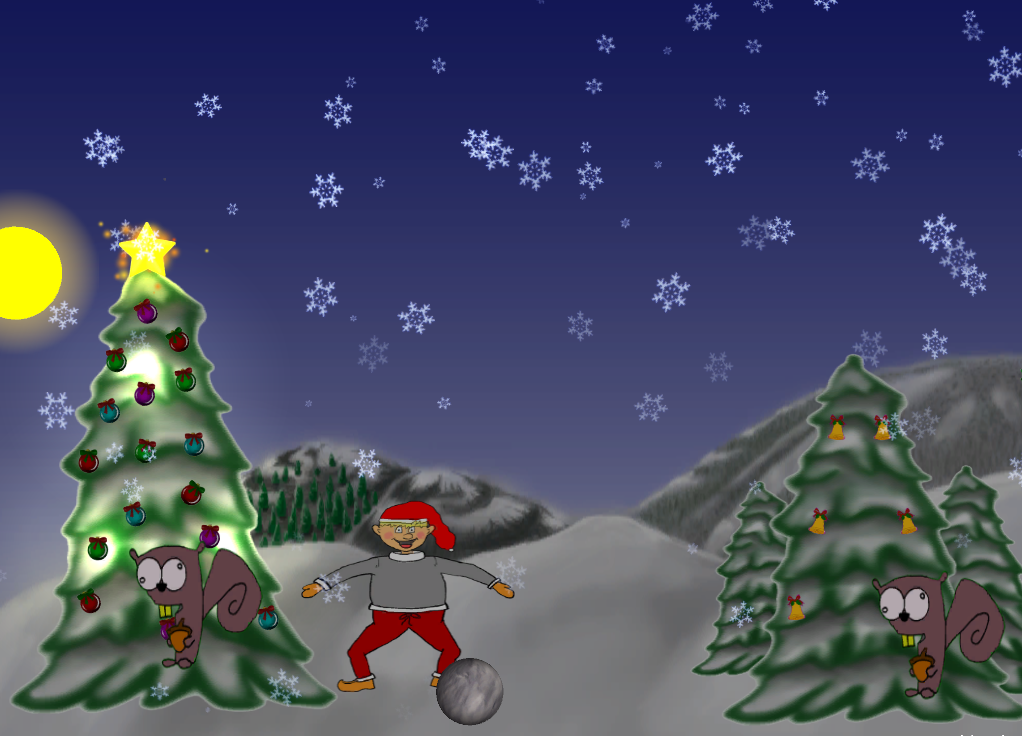
\includegraphics[width=1.00\textwidth]{Pictures/Design/time1.png} %Venstre billede
	\end{minipage}\hfill
	\begin{minipage}[b]{0.3\textwidth}\centering
		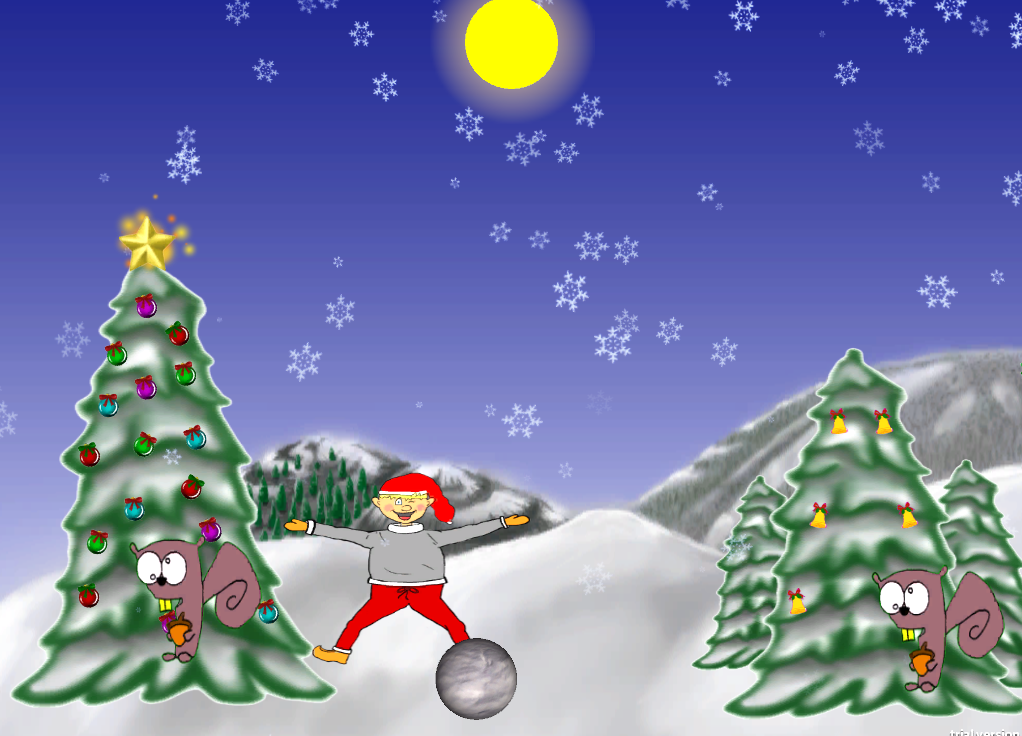
\includegraphics[width=1.00\textwidth]{Pictures/Design/time2.png} %Venstre billede
	\end{minipage}\hfill	
	\begin{minipage}[b]{0.3\textwidth}\centering
		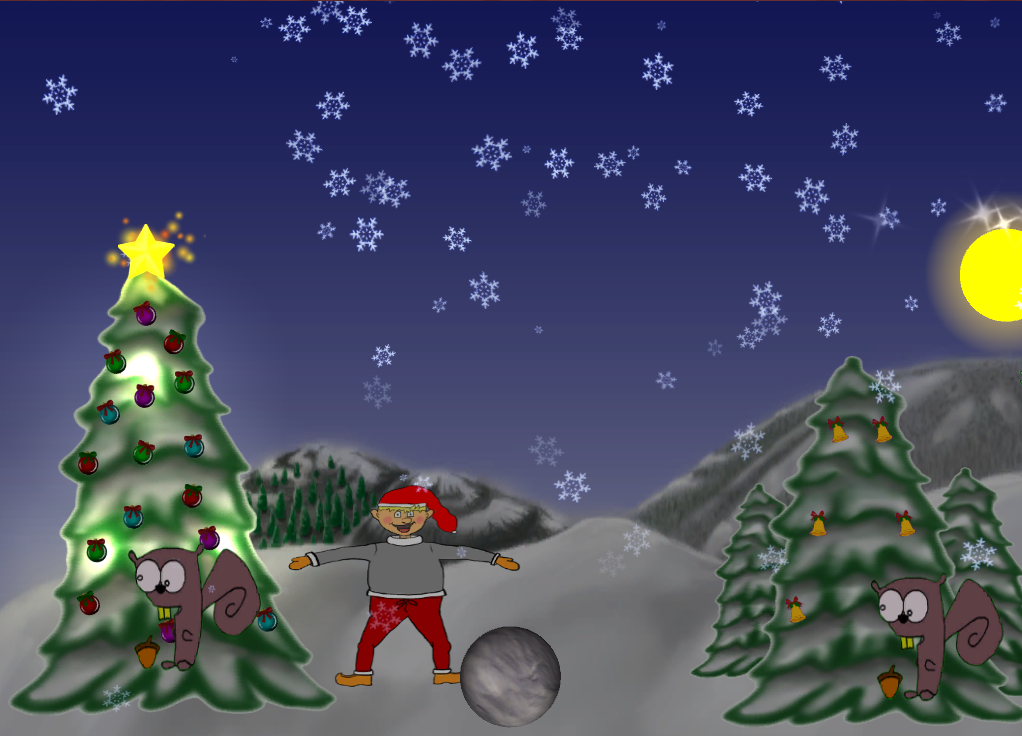
\includegraphics[width=1.00\textwidth]{Pictures/Design/time3.png} %Højre billede
	\end{minipage}\\ %Captions and labels
	\begin{minipage}[t]{0.3\textwidth}
		\caption{Morning.} %Venstre caption og label
		\label{fig:time1}
	\end{minipage}\hfill
	\begin{minipage}[t]{0.3\textwidth}
		\caption{Noon.} %Venstre caption og label
		\label{fig:time2}
	\end{minipage}\hfill	
	\begin{minipage}[t]{0.3\textwidth}
		\caption{Evening.} %Højre caption og label
		\label{fig:time3}
	\end{minipage}
\end{figure}

Another aspect is Santa Claus who will come at a randomly chosen time (see figure \ref{fig:santa}. When he arrives, jingle bell sounds play, as well as his iconic "ho ho ho" laughter. Santa will then drop packages that can be interacted with. This happens by moving into the objects, pushing them with the physics system in Unity. It should be noted that Santa doesn't come too often, since it would disturb other visitors at the library. In average, Santa Claus arrives once an hour.

\begin{figure}[htbp]
\centering
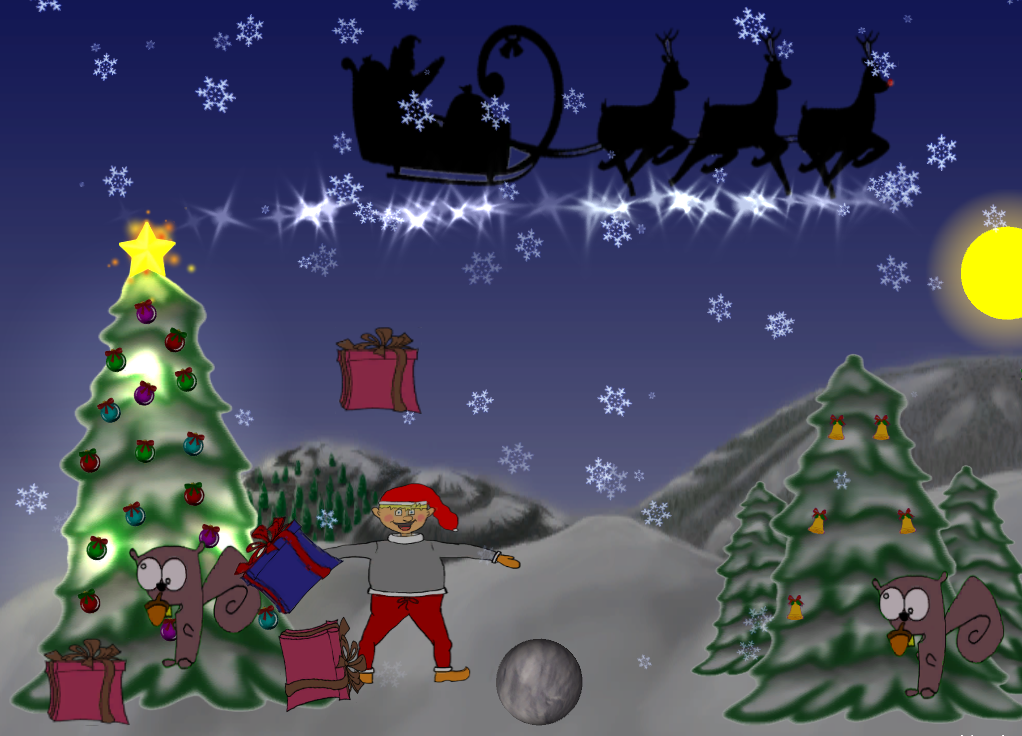
\includegraphics[width=0.90\textwidth]{Pictures/Design/santa.png}
\caption{Santa Claus comes at random times and drop presents. These can be pushed by the characters. They disappear after some time.}
\label{fig:santa}
\end{figure}

\subsection{Snow ball}
To get a little more interaction, a snow ball is placed in the scene (see figure \ref{fig:snowball}). This can be pushed around by the characters, and it will gradually grow bigger and bigger until it at some time explodes and disappear for a short period of time.


\begin{figure}[htbp]
\centering
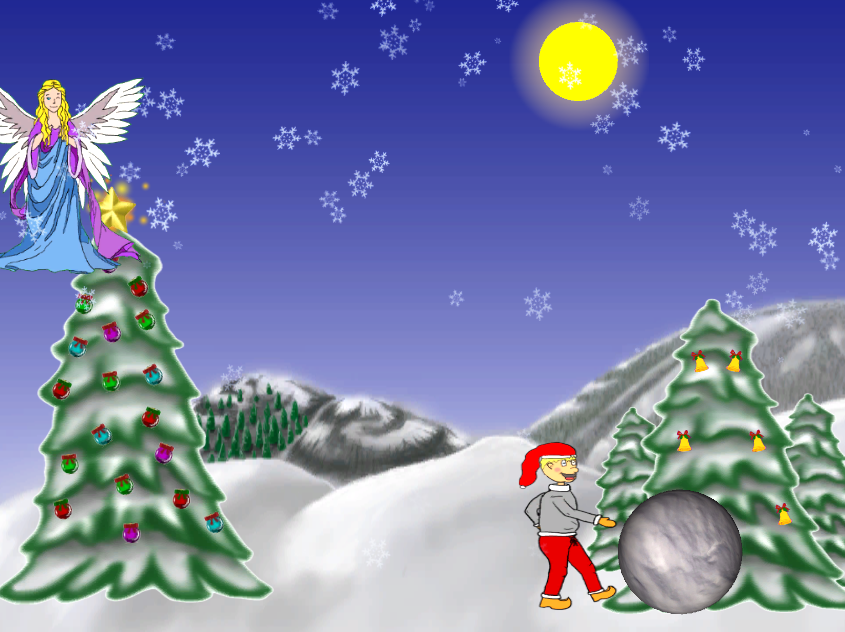
\includegraphics[width=0.90\textwidth]{Pictures/Design/pushing_snowball.png}
\caption{The characters can push the snowball to make it grow. When it becomes big enough, it explodes into colorful fireworks.}
\label{fig:snowball}
\end{figure}
As mentioned in \ref{spritesheet}, sheets of sprites were used to create a sense of motion. This was done by looping over an image containing multiple frames. Depending on which way the character is facing (left, right or idle), the animation will change. Without these animations the whole program would feel rigid and stiff.

\section{Making an automatic batch file}
One of the goals in the problem statement (\ref{problemStatement}) was to have the programs work as easily as possible. We could not expect the library staff to use a lot of time to turn everything on each day. Therefore we wanted everything to start automatically. This was done by creating a batch file that starts when Windows boots up. The batch file then opens the OpenCV program that initializes itself. After 15 seconds Unity opens and starts receiving data from the Clipboard. In the end, the only thing needed is just to turn on (and off) the computer; no additional input is required for the programs to start.

\section{Changes and limitations}
During the setup at the library multiple things were learned. Since it was not possible to be at Hj{\o}rring Library every day, especially not in the beginning of the project, it was difficult to test the proper camera settings, etc. Therefore we needed to re-adjust some elements when we visited the library.

\subsection{Use of LED strips}
The original plan was to be able to track people in front of and behind the bookshelf (dubbed "den r{\o}de tr{\aa}d). Therefore two sets of LED strips was put up: one behind the canvas (see figure \ref{fig:behindShelf}) and one beneath the red bookshelf (see figure \ref{fig:frontShelf}).

What the group hadn't have in mind was that the perspective that the camera would see (figure \ref{fig:camera_POV}). Since the program had already been written without this in mind, it was difficult to make it work with both LED strips. Due to lack of time it was decided to not use the LED strip in the background, but instead solely focus on the LED strip placed underneath the red bookshelf.

One thing that could be interesting to work on in the future would to be the background LED strip recognize hands. When trying out the program, it seemed intuitive to either jump or raise one's arms in the air. The LED strip could be used to track this, so the characters in the program could react accordingly. Sadly, there was no time to implement this idea.

\begin{figure}[htbp] \centering
\begin{minipage}[b]{0.45\textwidth} \centering
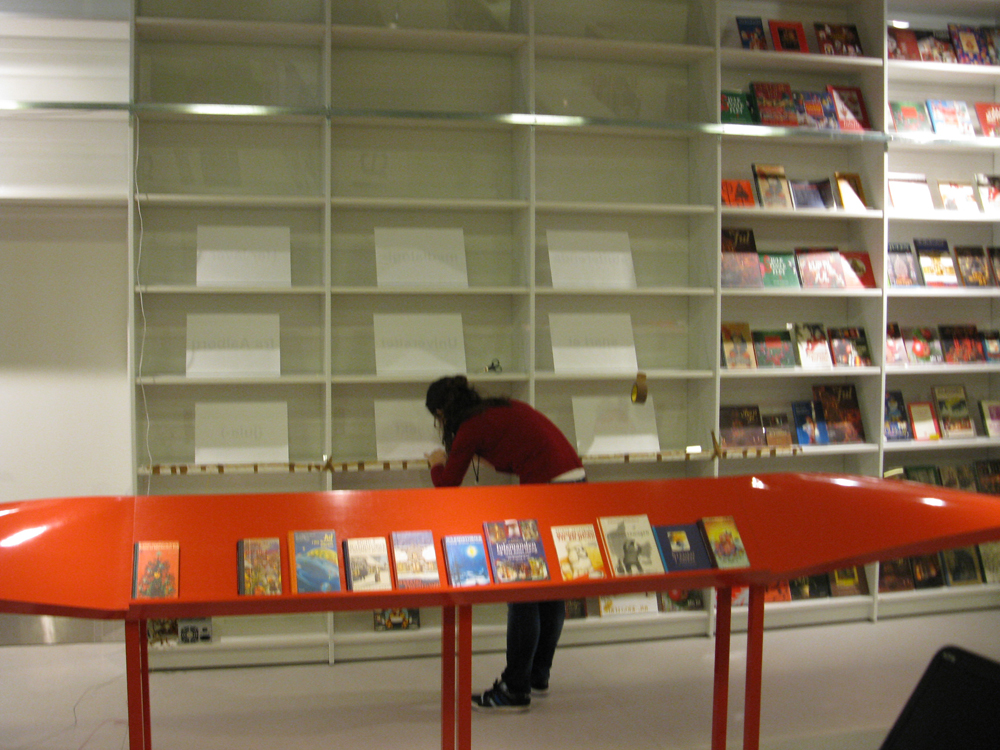
\includegraphics[width=1.00\textwidth]{Pictures/Design/behindShelf} % Venstre billede
\end{minipage} \hfill
\begin{minipage}[b]{0.45\textwidth} \centering
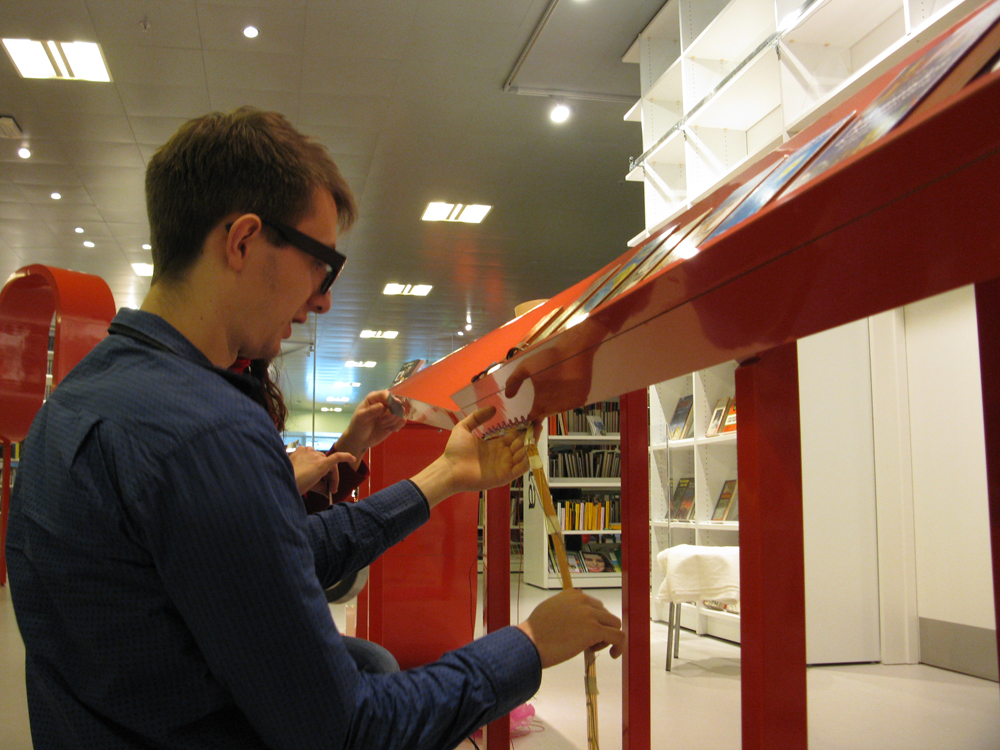
\includegraphics[width=1.00\textwidth]{Pictures/Design/frontShelf} % Højre billede
\end{minipage} \\ % Captions og labels
\begin{minipage}[t]{0.45\textwidth}
\caption{Behind bookshelf.} % Venstre caption og label
\label{fig:behindShelf}
\end{minipage} \hfill
\begin{minipage}[t]{0.45\textwidth}
\caption{Beneah bookshelf} % Højre caption og label
\label{fig:frontShelf}
\end{minipage}
\end{figure}

\begin{figure}[htbp]
\centering
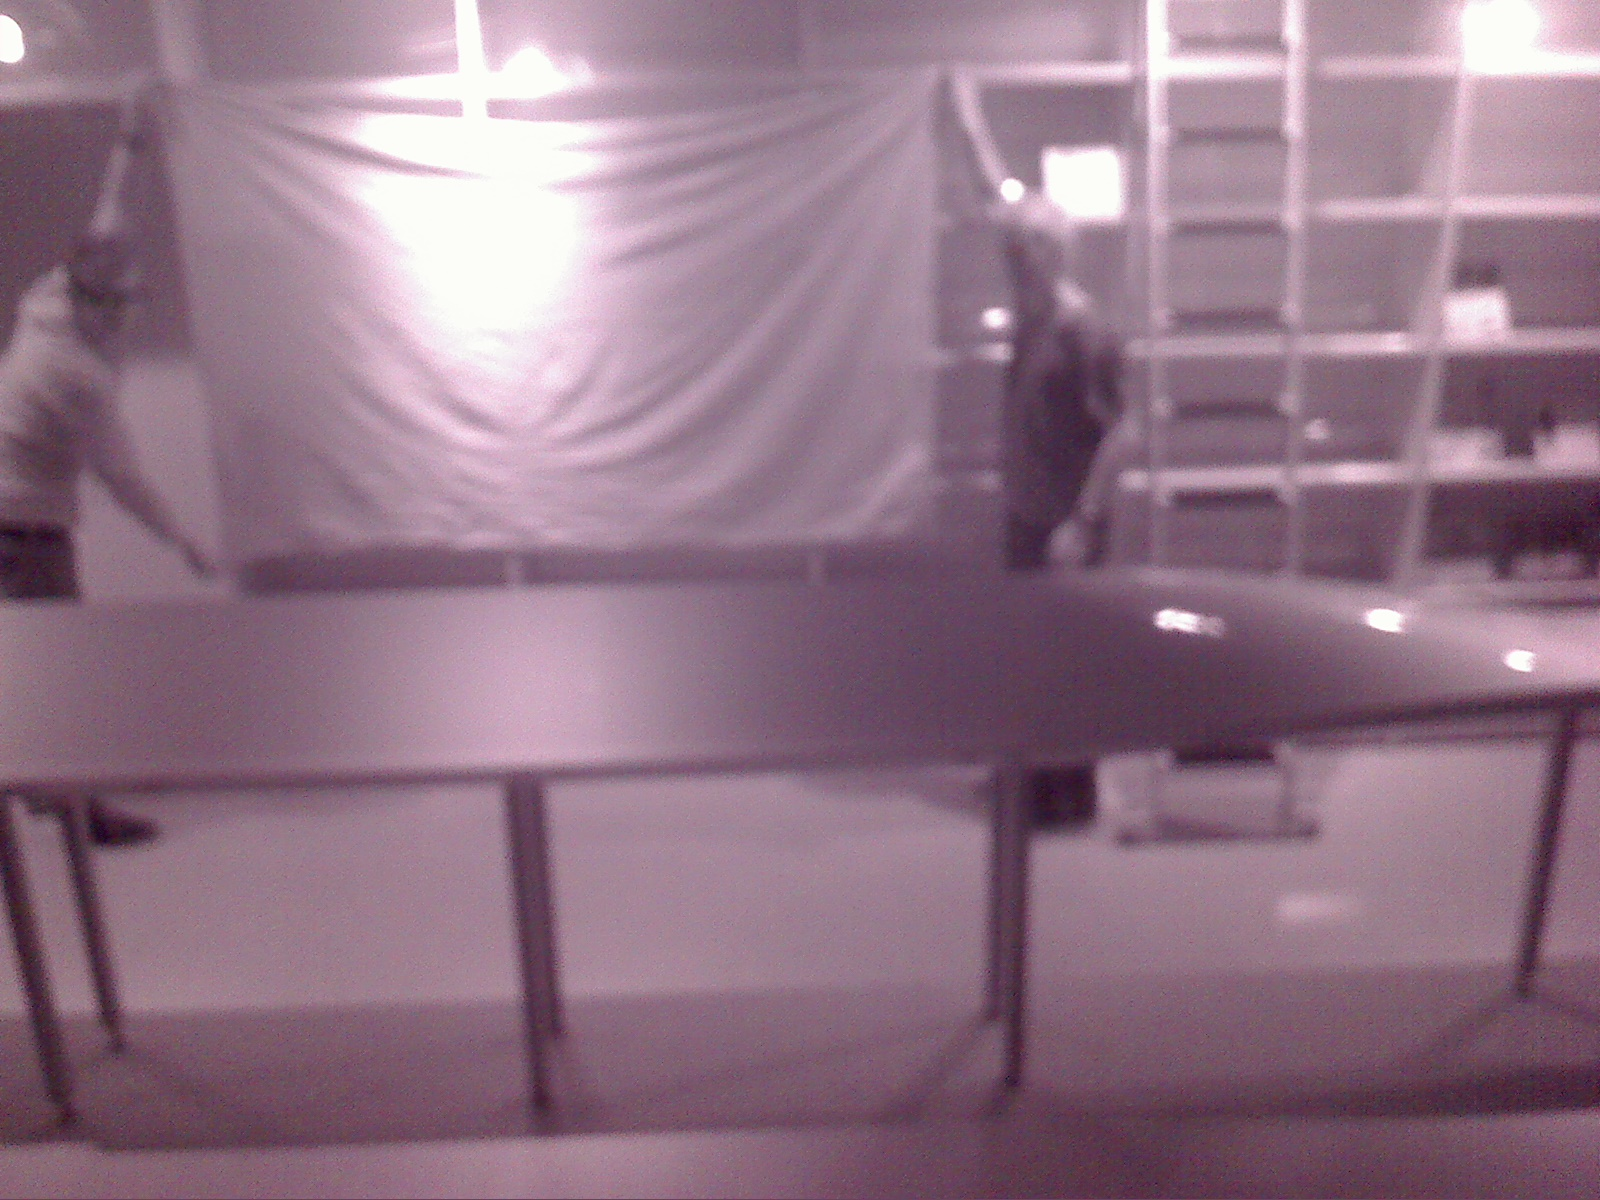
\includegraphics[width=0.70\textwidth]{Pictures/Design/IR_pic}
\caption{Camera point of view.}
\label{fig:camera_POV}
\end{figure}

\subsection{Santa Claus and his "ho ho ho" sound}
As mentioned previously, it was important not to disturb visitors with too much sound. After having the program running for a few hours, one of the library staff members contacted us and asked if it was our program that kept making weird noises. It turned out that she was talking about the Santa Claus "ho ho ho" laughter, which, in her opinion, sounded like a deep and growling voice. Apparently the speakers in that we were using made the "ho ho ho" sound different than on our laptop computers. The staff member said that it was a little disturbing and that she thought kids would be afraid, since it sounded a little creepy. On top of that, it sounded like she was a little annoyed of the sound, since she was working close-by.
In the end the group decided to just get rid of the sound and only use jingle bells for Santa's appearance.

\subsection{Shadows on canvas}
An unexpected problem was the fact that when somebody stand in front of the camera and projector, it draws a rather big shadow on the canvas. When the group first went to Hj{\o}rring to research and look for the location, it didn't seem like it would be a problem.

\textbf{[somebody, Johannes/Simon, needs to write a little more here!]}

\begin{figure}[htbp] \centering
\begin{minipage}[b]{0.45\textwidth} \centering
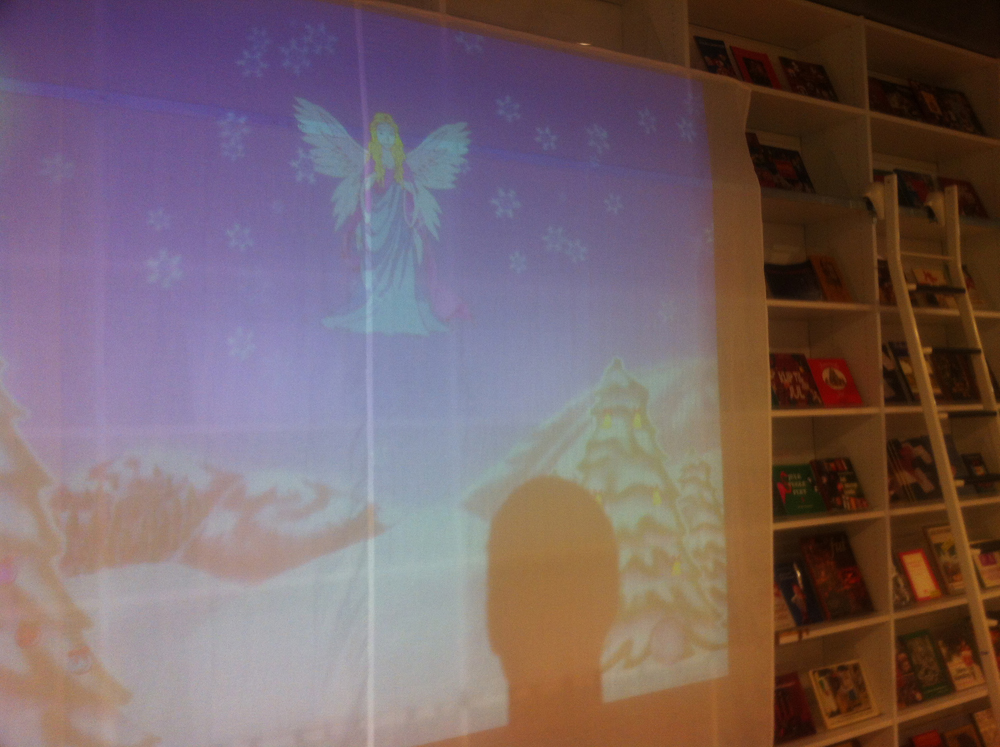
\includegraphics[width=1.00\textwidth]{Pictures/Design/shadow} % Venstre billede
\end{minipage} \hfill
\begin{minipage}[b]{0.45\textwidth} \centering
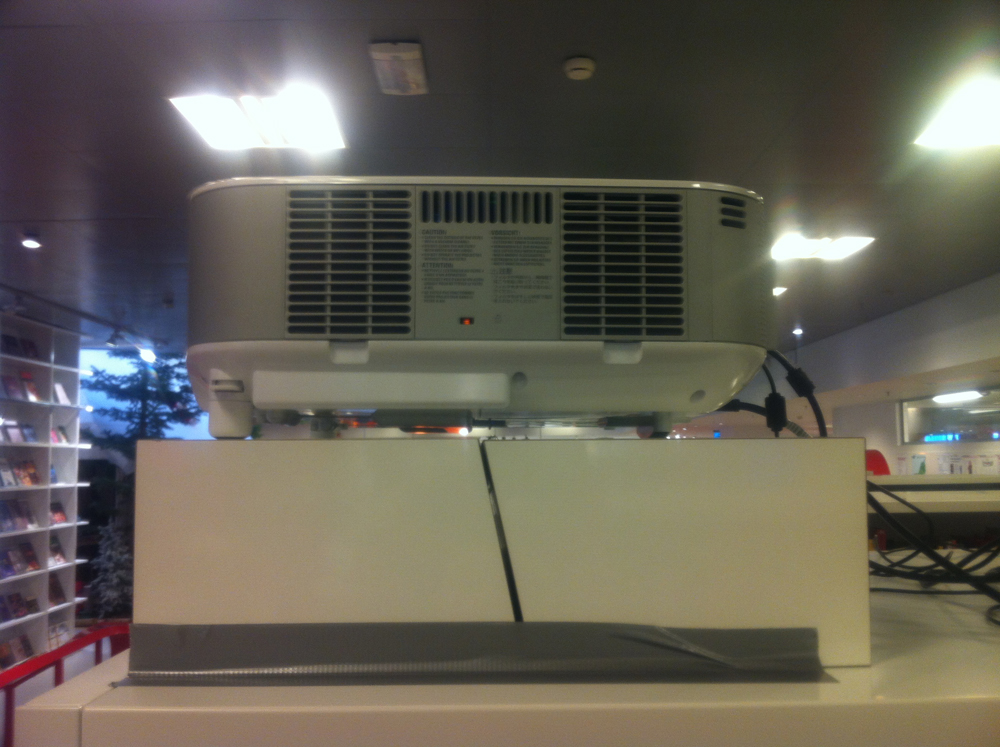
\includegraphics[width=1.00\textwidth]{Pictures/Design/projector_box} % Højre billede
\end{minipage} \\ % Captions og labels
\begin{minipage}[t]{0.45\textwidth}
\caption{If a visitor is standing too close to the red bookshelf, a shadow will cover the canvas.} % Venstre caption og label
\label{fig:shadow_canvas}
\end{minipage} \hfill
\begin{minipage}[t]{0.45\textwidth}
\caption{The projector needed to be placed higher to minimize shadows.} % Højre caption og label
\label{fig:projector_box}
\end{minipage}
\end{figure}

When the final setup was built, it turned out that in the worst-case scenario the shadow would hide a lot of the graphics drawn on the canvas (figure \ref{fig:shadow_canvas}). To reduce the shadows, the projector was placed on top of a couple of boxes (see figure \ref{fig:projector_box}). However, to completely remove the shadows one needed to use a lot of boxes, or, alternatively, hang the projector in the ceiling. Due to time constraints this was not possible. Also, the library staff was afraid that the projector would be too unstable.

\subsection{Need sound to draw attention}
One thing that the group quickly learned while setting the equipment up was the fact that a lot of people didn't even realize the fact that they were interacting with the canvas when the walked past. Many people looked straight forward when they were walking, instead of looking to either sides.

It was suggested to use sounds to draw attention to the canvas. An idea was to make a "magical fairy dust sound" play every time a person stepped into the scene. We tried this, but it didn't give a good result. One reasons was the fact that the speakers are placed inside the projector which is placed in the opposite side of the canvas. Figure \ref{fig:projector_audio} illustrates the problem.

\begin{figure}[htbp]
\centering
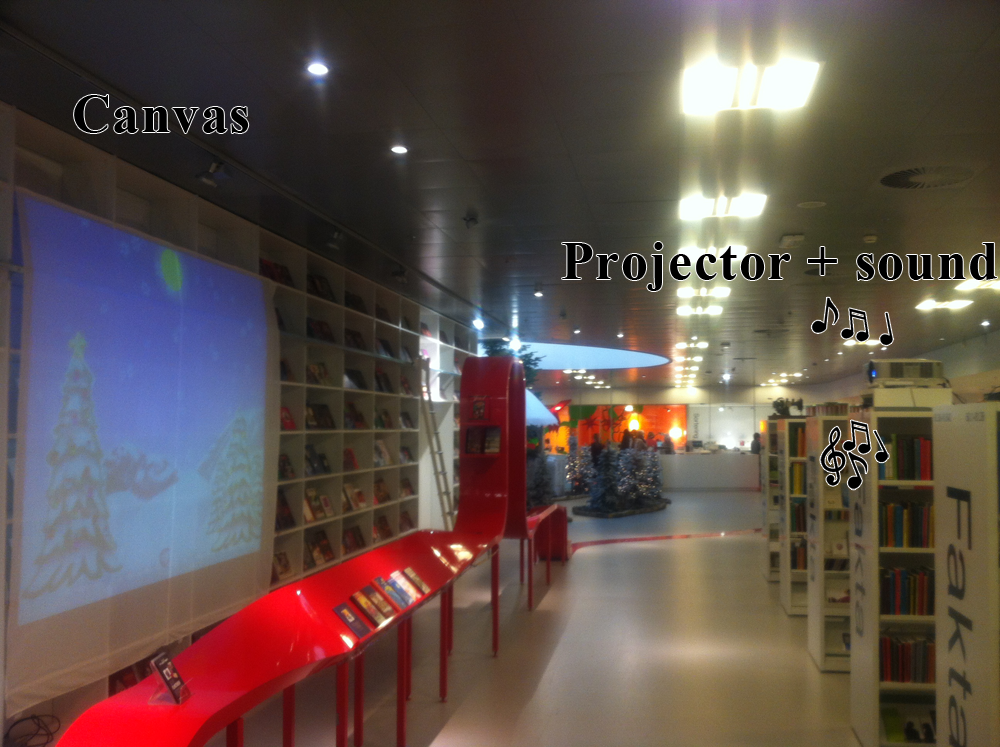
\includegraphics[width=1.0\textwidth]{Pictures/Design/projector_audio}
\caption{Since the speakers are inside the projector, audio will draw attention to the wrong side.}
\label{fig:projector_audio}
\end{figure}

The solution would be to place some external speakers near the canvas, but due to time constraints this wasn't implemented. Also, the sounds turned out to be a little disturbing, so in the end it was chosen to just drop them.

\subsection{People walking too fast}
Another reason why the canvas didn't draw proper attention when people walked past was the fact that it was quite slow to display the characters. In the beginning there was no real connection between a person walking and the character on-screen. This was due to multiple things: the camera having to process the data and send it to Unity, and the speed of the characters. It took some time for the characters to "cath up" on the actual person, so the character would be lagging behind. The solution was to teleport the character if the distance became too big.

\subsection{Camera not steady}
Initially there were some problems with the webcam moving just slightly. This would make the whole program malfunctioning, since the region of interest would change. To avoid this the webcam needed to be steadied with some strong tape. Also, the OpenCV program was modified to re-synchronize itself every hour. This would mean that if somebody accidentally touches either the camera or the LED strips (which happened surprisingly often), the program would re-adjust some time.

The group needed to make a decision: how often should it re-configure itself? If it did it too often, the chances of people standing in front of the camera while it was trying to re-configure was bigger. On the other hand, if it does it less often, the time where it won't work properly would be longer. In the end an hour was chosen to be a good compromise.

\textbf{[MAX should describe more why we chose an hour and not 2 hours, 5 hours, 5 min or something else!?]}

\subsection{Programs crashing during the day}
Before testing the program at the library, they hadn't run for more than a few minutes continuously. Since the goal was to let them run for a whole day (10:00-18:00), it was important that the programs would not crash. Initially, there were problems with both C++ and Unity.

\textbf{[something about C++ crashing]}

Even though the Unity program is quite simple, it turned out to hog a lot of memory over time. It took several days for the group to realize why. After multiple debugging sessions they found that apparently Unity does not deleted old textures and materials. As mentioned earlier, animations are done using sprite sheets. Doing this changes the material on a game object (a material describes how a texture should be displayed using a shader). Every time a new material is applied, i.e. when the animation needed to change, the old material was kept in the background. Over time, these materials stacked up. This meant that the RAM usage constantly increased until the program finally crashed.

To resolve this problem proper deletion of the materials were implemented. It turned out that the {C\#} garbage collector didn't do this automatically, so we manually had to delete old instances of materials. This lead to more stable memory usage. Just to be sure that Unity doesn't use too much memory during a whole day, it was made so that it reloads itself every third hour. This only takes a fraction of a second, so it shouldn't disturb the interaction.